% \begin{app}[Vectoriële kinematica]{Vectoriële kinematica}

% % \begin{itemize}
% %     \item $ \Vec{r} = r\Vec{u} $
% %     \item $ \Vec{v} = \dfrac{d\Vec{r}}{dt} $
% %     \item $ \Vec{a} = \dfrac{d\Vec{v}}{dt} = \dfrac{d^2\Vec{r}}{dt^2}$
% % \end{itemize}

% % % \vspace{0.5cm}

% % % \noindent Hieruit volgt dan logischerwijs ook: 

% % % \vspace{0.5cm}

% \centering
% \def\arraystretch{2.5}
% \begin{tabular}{c|c|c}
%      & $ \Vec{v} $ & $ \Vec{a} $ \\ \hline 
%      gem &  $ \Vec{v}_{gem} = \dfrac{\Delta \Vec{r}}{\Delta t} $ & $ \Vec{a}_{gem} = \dfrac{\Delta \Vec{v}}{\Delta t} $ \\ \hline
%      ogb & $ \Vec{v}  
%      % \lim_{\Delta t \to 0} \dfrac{\Delta \Vec{r}}{\Delta t}  
%      = \dfrac{d\Vec{r}}{dt}$ & $ \Vec{a} = 
%      % \lim_{\Delta t \to 0}\dfrac{\Delta \Vec{v}}{\Delta t} = 
%      \dfrac{d\Vec{v}}{dt} $ 
% \end{tabular}

% \end{app}

\begin{pro}[Nuttige vergelijkingen bij constante versnelling]{Nuttige vergelijkingen bij constante versnelling}

    De volgende vergelijkingen kunnen gebruikt worden wanneer de versnelling constant is: $a = \dfrac{dv}{dt} = cst$. 
    
    \begin{enumerate}
        \item $ r = r_{0} + v_{0}t + \tfrac{a}{2}t^2 = r_{0} + \overline{v}t$
        \item $ v = v_0 + at $ 
        \item $ \overline{v} = \dfrac{v + v_0}{2}$
        \item $ v^2 = v_0^2 + 2a(r-r_0) $
        % \begin{itemize}
        %     \item Dit kan je verkrijgen door (2) en (3) te substitueren in (1).
        % \end{itemize}
    \end{enumerate}
\end{pro}

\begin{app}[Projectielbeweging]{Projectielbeweging}

    Bij een projectielbeweging (zie figuur voor een projectielbeweging met $ v_{y,0} = 0 $) heeft het systeem horizontaal een constante snelheid (eenparige beweging) en verticaal een constante versnelling (eenparig versnelde beweging). In de volgende tabel zijn de formules samengevat: 
            
    \begin{minipage}{.43\textwidth}
    
        \def\arraystretch{2.5}
        \hspace{2cm}\begin{tabular}{c|c|c}
             & horizontaal & verticaal \\ \hline
             $ r $ & $ x_0 + v_{x,0}t $ & $ y_0 + v_{y,0}t - \dfrac{gt^2}{2} $ \\ \hline
             $ v $ & $ v_{x,0} $ & $ v_{y,0} - gt $  \\ \hline
             $ a $ & $ 0 $ & $ -g $ 
        \end{tabular}
        
    \end{minipage} 
    \begin{minipage}{.43\textwidth}
        \hspace{3cm}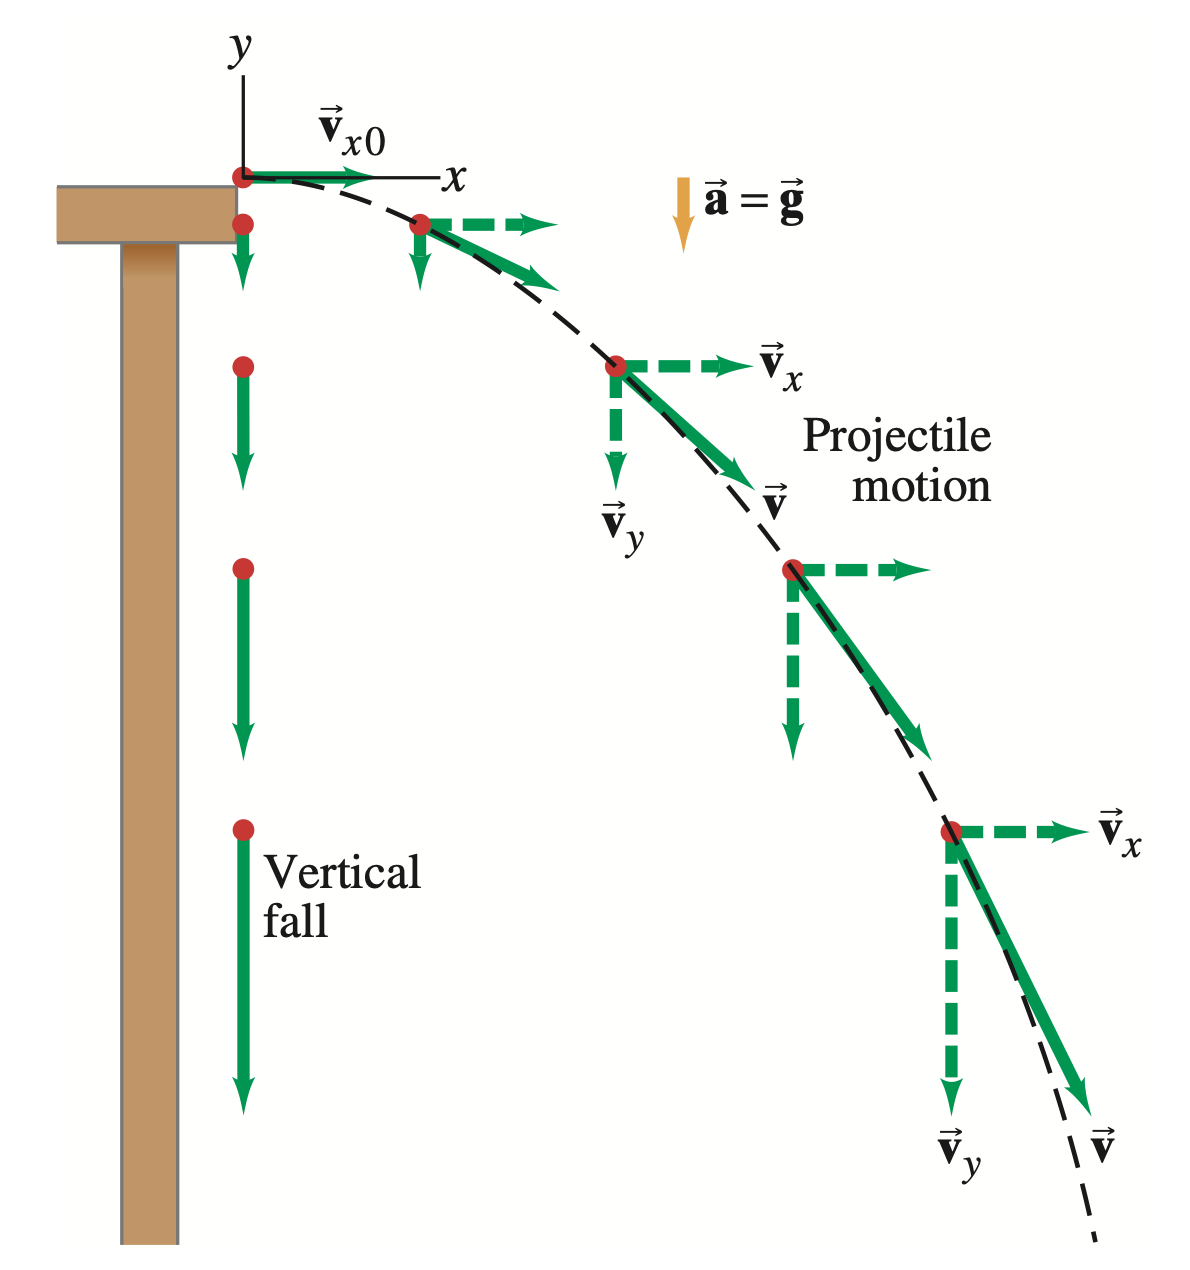
\includegraphics[scale = 0.25]{Images/Kinematica/Projectielbeweging.png}
    \end{minipage}
        
    \noindent Uit de voorgaande tabel kunnen we volgende formules halen: 
    
        \begin{equation*}
            x(t) = v_{x,0}t \to t = \dfrac{x(t)}{v_{x,0}}
        \end{equation*}
        
        \begin{equation*}
            y(t) = v_{y,0}t - \dfrac{gt^2}{2}
        \end{equation*}

    \vspace{0.25cm}
    \noindent Hieruit kunnen we de volgende formule bereiken:
    
    \begin{equation*}
        y(x) = \dfrac{v_{y,0}}{v_{x,0}}x - \dfrac{g}{2v_{x,0}^2}x^2
    \end{equation*}
    
    % \vspace{0.25cm}
    
    % Deze formule bepaald de volgende parabole projectielbaan:
    % \begin{center}
    %     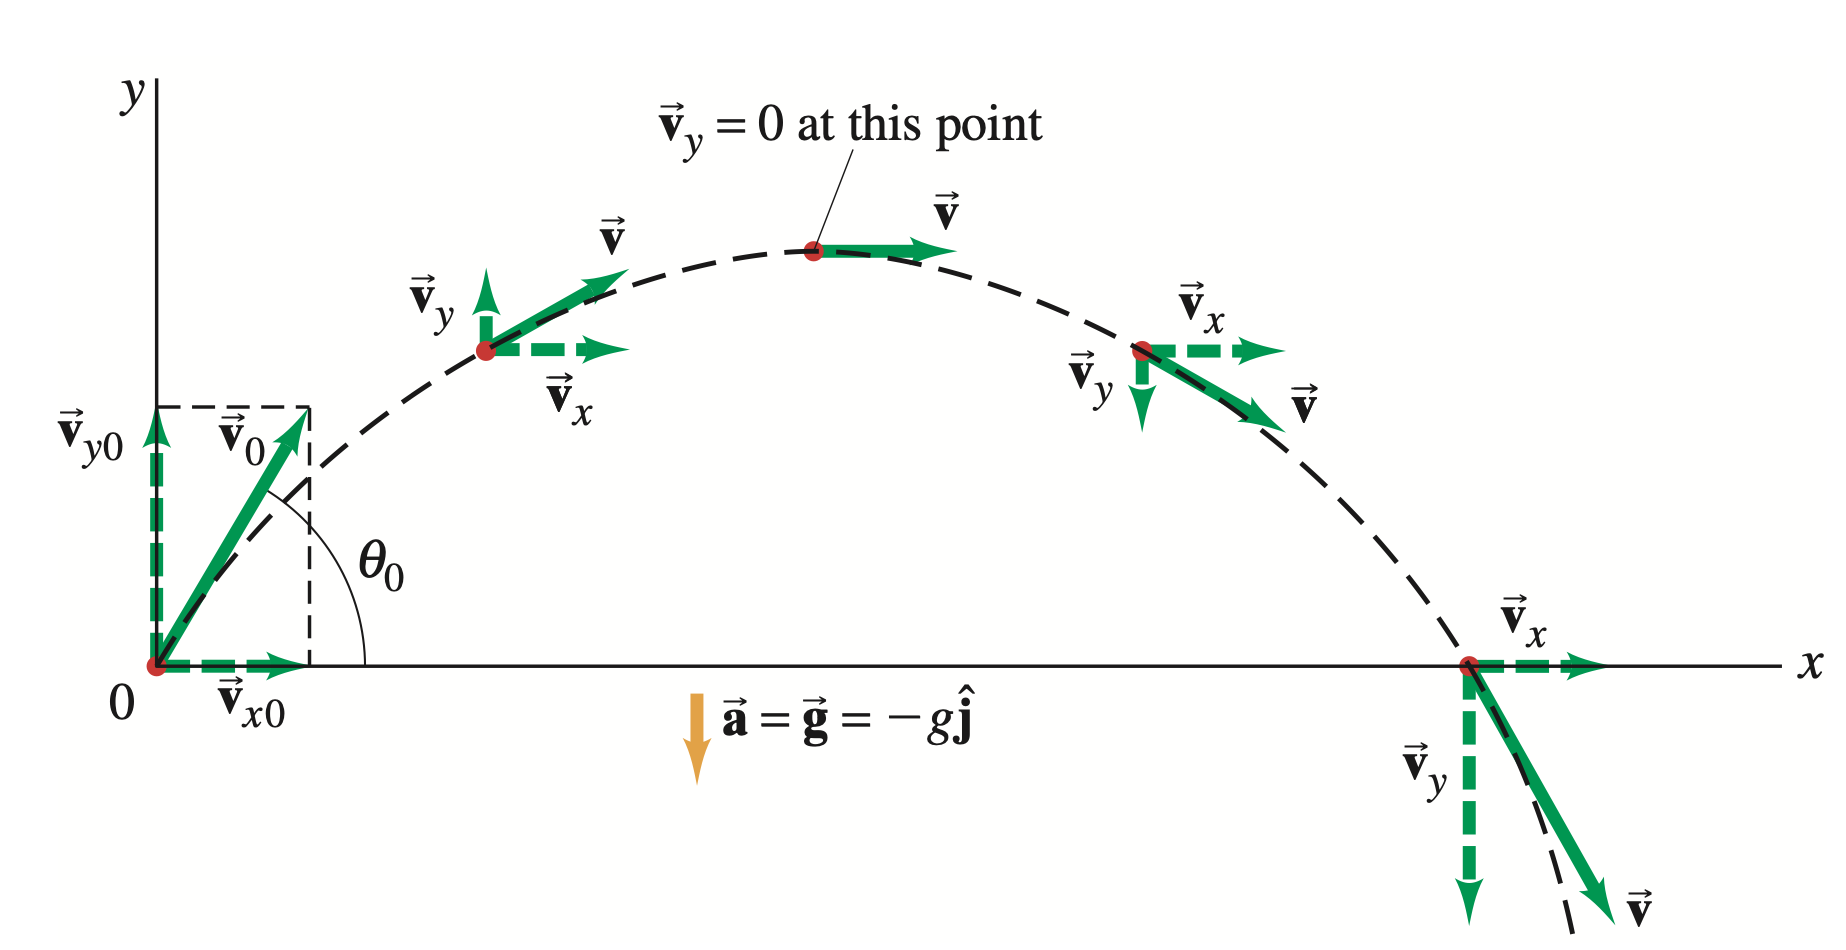
\includegraphics[scale = 0.325]{Images/Kinematica/Projectielbaan.png}
    % \end{center}
\end{app}
